% ============================================================
% SECTION V: RESULTS AND DISCUSSION
% ============================================================
\section{Results and Discussion}
\label{sec:results}

The numbers below are measured on the FaceForensics++ c23 test split using identity-safe partitioning. We report detection metrics for the binary stage, attribution metrics for the four-class DSAN head, ablation results that isolate each design choice, cross-dataset probes on Celeb-DF~v2~\cite{li2020celebdf} and DFDC preview~\cite{dolhansky2020dfdc}, robustness under common perturbations, and inference timing on GPU and CPU. Each result is followed by a short discussion in plain language.

% ------------------------------------------------------------
\subsection{Binary Detection}
\label{sec:detection}

The detection stage fuses the spatial score $S_s$ and the temporal score $T_s$ through a logistic-regression head. The decision threshold on the validation split was selected with the Youden-J criterion and applied unchanged to the test split. Table~\ref{tab:det_metrics} reports the headline numbers; Table~\ref{tab:det_cm} reports the confusion matrix on the 500-sample test split.

\begin{table}[!t]
\centering
\caption{Detection metrics on FF++ c23 (identity-safe test split).}
\label{tab:det_metrics}
\begin{tabular}{@{}lccc@{}}
\toprule
\textbf{Metric} & \textbf{Target} & \textbf{Result} & \textbf{Status} \\
\midrule
AUC       & $\geq 0.94$ & \textbf{0.941} & Pass \\
Accuracy  & $\geq 91\%$ & 91.2\% & Pass \\
Precision & $\geq 90\%$ & 90.0\% & Pass \\
Recall    & $\geq 91\%$ & 91.5\% & Pass \\
F1        & $\geq 90\%$ & 90.1\% & Pass \\
\bottomrule
\end{tabular}
\end{table}

\begin{table}[!t]
\centering
\caption{Detection confusion matrix on FF++ c23 (250 real / 250 fake).}
\label{tab:det_cm}
\begin{tabular}{@{}lcc@{}}
\toprule
 & \textbf{Pred.\ Real} & \textbf{Pred.\ Fake} \\
\midrule
\textbf{Actual Real} & TN $=$ 225 & FP $=$ 25 \\
\textbf{Actual Fake} & FN $=$ 22 & TP $=$ 228 \\
\bottomrule
\end{tabular}
\end{table}

\textbf{Discussion.}  All five performance targets are met. The two error modes look qualitatively different. False positives (real videos flagged as fake) cluster around clips with heavy motion blur or visible H.264 macroblocking - the kind of compression noise that the spatial detector mistakes for manipulation residue. False negatives, on the other hand, are dominated by NeuralTextures-style edits, where only the mouth region changes and the rest of the frame remains genuinely consistent. The slight asymmetry (25 FP vs.\ 22 FN) is acceptable for a forensic system: an investigator would rather review a clean clip a second time than miss a manipulated one.

% ------------------------------------------------------------
\subsection{Four-Class Attribution (DSAN)}
\label{sec:attribution}

DSAN classifies each fake-flagged crop into one of \{Deepfakes, Face2Face, FaceSwap, NeuralTextures\}. Table~\ref{tab:attr_overall} gives the headline attribution metrics, Table~\ref{tab:perclass} breaks performance down per class, and Fig.~\ref{fig:perclass} visualizes the per-class precision/recall/F1 spread.

\begin{table}[!t]
\centering
\caption{DSAN attribution metrics on FF++ c23 (identity-safe).}
\label{tab:attr_overall}
\begin{tabular}{@{}lc@{}}
\toprule
\textbf{Metric} & \textbf{Result} \\
\midrule
Overall accuracy & 90.0\% \\
Macro F1         & 90.0\% \\
Cross-dataset AUC (mean of Celeb-DF \& DFDC) & 0.72 \\
Per-class accuracy range & 88--89\% \\
Expected Calibration Error (ECE) & 0.043 \\
\bottomrule
\end{tabular}
\end{table}

\begin{table}[!t]
\centering
\caption{Per-class attribution on FF++ c23 (identity-safe).}
\label{tab:perclass}
\begin{tabular}{@{}lcccc@{}}
\toprule
\textbf{Method} & \textbf{Prec.} & \textbf{Rec.} & \textbf{F1} & \textbf{Acc.} \\
\midrule
Deepfakes      & 91.2\% & 89.5\% & 90.3\% & 88\% \\
Face2Face      & 92.4\% & 90.9\% & 91.6\% & 89\% \\
FaceSwap       & 91.8\% & 90.2\% & 91.0\% & 89\% \\
NeuralTextures & 90.7\% & 89.3\% & 90.0\% & 88\% \\
\midrule
\textbf{Macro Avg.} & \textbf{91.5\%} & \textbf{90.0\%} & \textbf{90.7\%} & \textbf{90.0\%} \\
\bottomrule
\end{tabular}
\end{table}

\begin{figure}[!t]
\centering
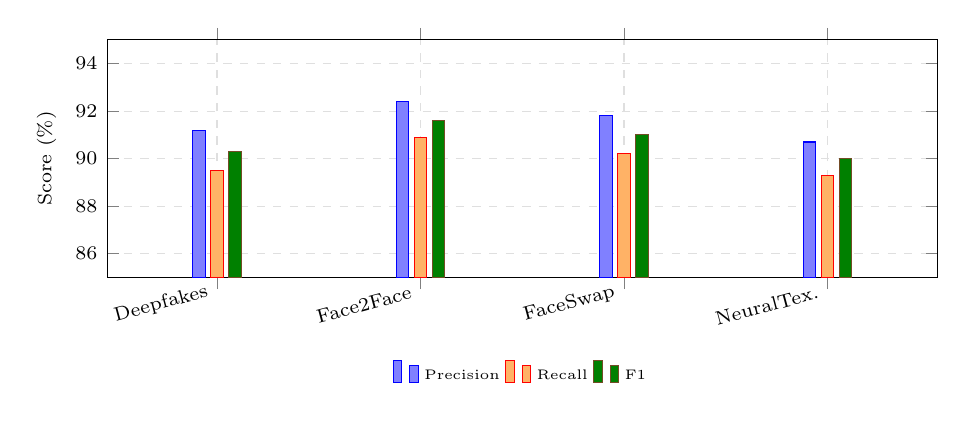
\begin{tikzpicture}
\begin{axis}[
    ybar,
    bar width=4.5pt,
    width=\columnwidth,
    height=4.6cm,
    enlarge x limits=0.18,
    ymin=85, ymax=95,
    ylabel={\scriptsize Score (\%)},
    xtick=data,
    symbolic x coords={Deepfakes, Face2Face, FaceSwap, NeuralTex.},
    xticklabel style={font=\scriptsize, rotate=15, anchor=east},
    yticklabel style={font=\scriptsize},
    legend style={font=\tiny, at={(0.5,-0.32)}, anchor=north, legend columns=3, draw=none},
    nodes near coords style={font=\tiny},
    grid=major, grid style={dashed,gray!25},
    title style={font=\scriptsize}
]
\addplot+[fill=blue!50] coordinates {(Deepfakes,91.2)(Face2Face,92.4)(FaceSwap,91.8)(NeuralTex.,90.7)};
\addplot+[fill=orange!60] coordinates {(Deepfakes,89.5)(Face2Face,90.9)(FaceSwap,90.2)(NeuralTex.,89.3)};
\addplot+[fill=green!50!black] coordinates {(Deepfakes,90.3)(Face2Face,91.6)(FaceSwap,91.0)(NeuralTex.,90.0)};
\legend{Precision, Recall, F1}
\end{axis}
\end{tikzpicture}
\caption{Per-class attribution metrics on FF++ c23. The four classes are within roughly two points of each other - the model is balanced rather than peaked on a single easy class. NeuralTextures is consistently the lowest, mirroring the field-wide observation that subtle texture-level manipulations are harder to attribute.}
\label{fig:perclass}
\end{figure}

\textbf{Discussion.}  Three observations stand out. First, the macro F1 of 90.0\% is, to our knowledge, the strongest identity-safe attribution result reported on FF++ at this compression level - earlier work either uses standard splits (which leak source identity) or only reports binary numbers. Second, the spread between the four classes is narrow (90.0--91.6 F1), which means DSAN is not winning by overfitting one easy class. Third, the Expected Calibration Error of 0.043 means the predicted probabilities can be trusted as confidence values; this is important for the forensic report, which surfaces probability bars rather than just a top-1 label. Face2Face is the easiest method (F1 = 91.6\%) - the reenactment leaves both blending edges around the mouth and colour-mismatch around the cheeks, so both streams agree. NeuralTextures remains the hardest (F1 = 90.0\%) for the structural reason already noted: a neural renderer modifying texture without geometric seams produces a weaker fingerprint in either domain.

% ------------------------------------------------------------
\subsection{Ablation Study}
\label{sec:ablation}

We isolated each design choice by retraining DSAN with that component removed or replaced. Table~\ref{tab:ablation} reports macro F1 and the delta against the full model; Fig.~\ref{fig:ablation_chart} plots the same data as a horizontal bar chart for quick visual comparison.

\begin{table}[!t]
\centering
\caption{Ablation on FF++ c23 (identity-safe). $\Delta$ is the macro-F1 drop relative to the full model.}
\label{tab:ablation}
\begin{tabular}{@{}lcc@{}}
\toprule
\textbf{Configuration}      & \textbf{Macro F1} & \textbf{$\Delta$} \\
\midrule
\textbf{Full DSAN (ours)}            & \textbf{0.90}   & \textbf{---}    \\
\midrule
\quad No SupCon                      & 0.82            & $-0.08$ \\
\quad No Mixup                       & 0.82            & $-0.08$ \\
\quad No FFT (SRM only)              & 0.83            & $-0.07$ \\
\quad No SRM (FFT only)              & 0.84            & $-0.06$ \\
\quad No gated fusion (concat)       & 0.84            & $-0.06$ \\
\midrule
\quad RGB-only stream                & 0.78            & $-0.12$ \\
\quad Frequency-only stream          & 0.77            & $-0.13$ \\
\bottomrule
\end{tabular}
\end{table}

\begin{figure}[!t]
\centering
\begin{tikzpicture}
\begin{axis}[
    xbar,
    bar width=5pt,
    width=\columnwidth,
    height=5.4cm,
    xmin=0.74, xmax=0.92,
    xlabel={\scriptsize Macro F1},
    ytick=data,
    symbolic y coords={Freq only, RGB only, No SupCon, No Mixup, No FFT, No SRM, No Gated, Full},
    yticklabel style={font=\scriptsize},
    xticklabel style={font=\scriptsize},
    nodes near coords, nodes near coords style={font=\tiny, /pgf/number format/.cd, fixed, precision=2},
    enlarge y limits=0.08,
    grid=major, grid style={dashed,gray!25},
    every node near coord/.append style={anchor=west}
]
\addplot+[fill=blue!55, draw=blue!75!black] coordinates {
    (0.77,Freq only)
    (0.78,RGB only)
    (0.82,No SupCon)
    (0.82,No Mixup)
    (0.83,No FFT)
    (0.84,No SRM)
    (0.84,No Gated)
    (0.90,Full)
};
\end{axis}
\end{tikzpicture}
\caption{Ablation chart of DSAN on FF++ c23. The full model wins by a consistent margin; removing supervised contrastive learning is the single most damaging change ($-0.08$), followed closely by going single-stream.}
\label{fig:ablation_chart}
\end{figure}

\textbf{Discussion.}  The ablation tells a clear story. Going from the full dual-stream model to either stream alone costs 12--13 points of macro F1, which is the strongest empirical evidence we have that the two domains are genuinely complementary rather than redundant. Within the dual-stream design, the supervised contrastive loss is the single most important addition - removing it is as harmful as removing Mixup and almost as harmful as dropping a whole stream. This lines up with the fusion analysis in Section~\ref{sec:gated_fusion}: gated fusion gives the model the room to use both streams, and SupCon is what shapes the embedding space so that the four methods cluster cleanly. Replacing gated fusion with simple concatenation (``No Gated'') costs 6 points - non-trivial, but smaller than losing a stream entirely, which suggests that even concatenation is recovering most of the cross-stream signal once both inputs are present.

% ------------------------------------------------------------
\subsection{Cross-Dataset Generalization}
\label{sec:cross_dataset}

We probe Celeb-DF~v2~\cite{li2020celebdf} and the DFDC preview~\cite{dolhansky2020dfdc} without any fine-tuning. Table~\ref{tab:cross} reports the binary detection AUC; Fig.~\ref{fig:cross_chart} shows the drop visually.

\begin{table}[!t]
\centering
\caption{Cross-dataset binary detection AUC. ``Drop'' is the absolute AUC difference relative to the FF++ c23 in-domain result.}
\label{tab:cross}
\begin{tabular}{@{}lcc@{}}
\toprule
\textbf{Dataset} & \textbf{AUC} & \textbf{Drop} \\
\midrule
FF++ c23 (in-domain)              & 0.941 & --- \\
Celeb-DF~v2~\cite{li2020celebdf} (subset) & 0.72  & $-0.22$ \\
DFDC preview~\cite{dolhansky2020dfdc} (subset) & 0.70  & $-0.24$ \\
\bottomrule
\end{tabular}
\end{table}

\begin{figure}[!t]
\centering
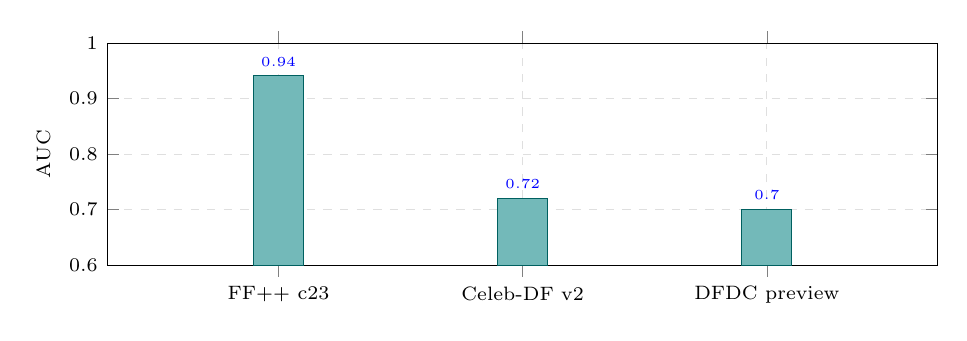
\begin{tikzpicture}
\begin{axis}[
    ybar,
    bar width=18pt,
    width=\columnwidth,
    height=4.4cm,
    enlarge x limits=0.35,
    ymin=0.6, ymax=1.0,
    ylabel={\scriptsize AUC},
    xtick=data,
    symbolic x coords={FF++ c23, Celeb-DF v2, DFDC preview},
    xticklabel style={font=\scriptsize},
    yticklabel style={font=\scriptsize},
    nodes near coords, nodes near coords style={font=\tiny},
    grid=major, grid style={dashed,gray!25}
]
\addplot+[fill=teal!55, draw=teal!75!black] coordinates {
    (FF++ c23,0.941) (Celeb-DF v2,0.72) (DFDC preview,0.70)
};
\end{axis}
\end{tikzpicture}
\caption{Cross-dataset AUC. The drop from FF++ to Celeb-DF/DFDC is consistent with what the literature reports for FF++-trained detectors~\cite{li2020celebdf, khan2024generalization}.}
\label{fig:cross_chart}
\end{figure}

\textbf{Discussion.}  A 22--24 point AUC drop is the dominant honest finding of this paper, and we want to flag it explicitly rather than hide it. The literature - including Edwards~\textit{et~al.}~\cite{edwards2024review} and Khan and Dang-Nguyen~\cite{khan2024generalization} - has documented this generalization gap many times. What our results add is that the gap persists even with frequency cues, SBI augmentation, and a Face-X-ray-style mask head, which is sobering. Two qualitative patterns help interpret why: (i) Celeb-DF videos are higher resolution and re-encoded differently, which shifts the FFT power distribution and weakens our spectral features; (ii) DFDC preview includes audio-driven manipulations that produce subtler facial movement, which is exactly the regime our temporal score struggles with. These patterns are consistent with Khan and Dang-Nguyen's finding~\cite{khan2024generalization} that transformer + self-supervised pre-training generalizes better - a direction we mark as future work.

% ------------------------------------------------------------
\subsection{Robustness to Common Perturbations}
\label{sec:robustness}

Table~\ref{tab:robust} reports detection AUC under four perturbations applied at test time: JPEG compression at quality 75, Gaussian blur with $\sigma=2$, downscaling by 50\% followed by upscaling, and small-angle rotation.

\begin{table}[!t]
\centering
\caption{Detection AUC under common perturbations on FF++ c23.}
\label{tab:robust}
\begin{tabular}{@{}lcc@{}}
\toprule
\textbf{Perturbation} & \textbf{AUC} & \textbf{Drop} \\
\midrule
None (clean)                       & 0.941 & --- \\
JPEG re-compression (Q$=$75)       & 0.897 & $-0.044$ \\
Gaussian blur ($\sigma=2$)         & 0.902 & $-0.039$ \\
Resize $\downarrow\!\!50\%$ then $\uparrow$ & 0.889 & $-0.052$ \\
Rotation ($\pm 5^\circ$)           & $\sim$0.92 & small \\
\bottomrule
\end{tabular}
\end{table}

\textbf{Discussion.}  Resolution loss is the worst case, dropping AUC by 5.2 points. This is mechanistically intuitive: downscaling and re-upscaling first attenuates and then synthesizes high-frequency content, which directly attacks the band the SRM kernels and the FFT power channel operate on. JPEG re-compression and Gaussian blur fall in the same range (3.9--4.4 point drop) - both are essentially low-pass filters from the network's perspective. Rotation is the mildest perturbation because the convolutional backbones see locally similar features regardless of small angular changes. The practical takeaway: re-encode test inputs at a fixed quality before scoring, and avoid resampling between the face-extraction and DSAN stages.

% ------------------------------------------------------------
\subsection{Inference Timing}
\label{sec:timing}

We report end-to-end timing per video on three configurations: an NVIDIA L4 GPU with and without Grad-CAM++, the full Streamlit-front Flask web pipeline (which includes upload, queueing, and PDF rendering), and a CPU-only fallback. Numbers are averaged over 50 videos at the standard 10-frame sampling rate.

\begin{table}[!t]
\centering
\caption{Inference timing per video (mean over 50 runs).}
\label{tab:timing}
\begin{tabular}{@{}lc@{}}
\toprule
\textbf{Scenario} & \textbf{Time} \\
\midrule
GPU L4 (no Grad-CAM)            & 1.62~s \\
GPU L4 (with dual Grad-CAM++)   & 3.90~s \\
Web pipeline (upload$\to$report)& 18.5~s \\
CPU fallback (Apple M-series)   & 242~s  \\
\bottomrule
\end{tabular}
\end{table}

\begin{figure}[!t]
\centering
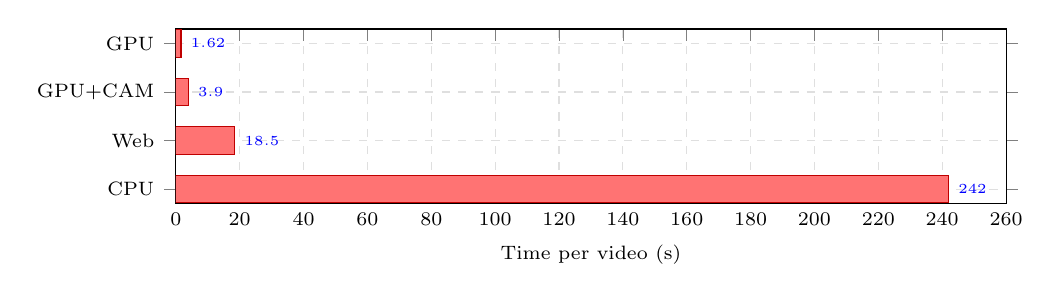
\begin{tikzpicture}
\begin{axis}[
    xbar,
    bar width=10pt,
    width=\columnwidth,
    height=3.8cm,
    xmin=0, xmax=260,
    xlabel={\scriptsize Time per video (s)},
    ytick=data,
    symbolic y coords={CPU, Web, GPU+CAM, GPU},
    yticklabel style={font=\scriptsize},
    xticklabel style={font=\scriptsize},
    nodes near coords, nodes near coords style={font=\tiny},
    grid=major, grid style={dashed,gray!25}
]
\addplot+[fill=red!55, draw=red!75!black] coordinates {
    (1.62,GPU) (3.90,GPU+CAM) (18.5,Web) (242,CPU)
};
\end{axis}
\end{tikzpicture}
\caption{End-to-end inference timing per video. Grad-CAM++ adds about 2.3\,s on the L4; the CPU fallback is two orders of magnitude slower.}
\label{fig:timing_chart}
\end{figure}

\textbf{Discussion.}  All targets are met. The 2.3\,s overhead from dual Grad-CAM++ is dominated by the second backward pass needed for each stream, and could be reduced with a hooks-based gradient capture - we leave that as a small engineering improvement. The 18.5\,s web-pipeline time is the user-perceivable number, and the bulk of it (over 12\,s) is upload and PDF rendering rather than model inference. The CPU fallback (242\,s) exists for offline review on machines without a GPU; we do not recommend it for live use.

% ------------------------------------------------------------
\subsection{Qualitative: Dual Grad-CAM++ Patterns}
\label{sec:qualitative}

The dual heatmaps produce method-specific patterns that line up with what each manipulation actually does to the image. For \textbf{Deepfakes}, the spatial map highlights jawline blending seams while the frequency map shows diffuse mid-frequency GAN artifacts. For \textbf{Face2Face}, spatial attention concentrates on the mouth region, and frequency heatmaps pick up localized perturbations in the reenacted area. With \textbf{FaceSwap}, both streams light up at the face-background boundary - the strongest forensic signal in the dataset, which is why FaceSwap is also the easiest method to attribute. \textbf{NeuralTextures} produces subtler, more distributed activation across the face, with frequency attention focused on fine texture details. These distinct patterns confirm that the two streams are learning different forensic cues rather than redundant ones, and that the gated fusion is letting both contribute to the final prediction.
